\section{Numerical study}\label{sec:experiments}

\subsection{Setup}

All experiments use Bernoulli rewards, which lie in $[0,1]$ and are therefore $1/4$-, hence $1$-sub-Gaussian, so every bound of Sections~\ref{sec:hoeffding}--\ref{sec:noise} applies. The bandit runs for $T=30{,}000$ rounds with $\tau_1=10{,}000$ and $\tau_2=20{,}000$; each configuration is replicated $200$ times with seeded random streams. The simulator (\texttt{src/cpbandits.py}) vectorizes the replications and keeps, for each arm, a ring buffer of its last $w$ observations together with the phase in which each was collected, so the stale fractions $\alpha_{i,k}(t)$ of \eqref{eq:alpha} are available exactly. Its window statistics are checked against a direct recomputation in the unit tests.

\paragraph{Policies.} In the first phase all policies run the UCB rule \eqref{eq:ucb} with $\delta=\tau_1^{-2}$. After $\tau_1$ they use the window estimator of part~(c) with the radius $r(m)=\sqrt{2L_T/m}$, $\delta=1/T$, in one of four variants:
\begin{itemize}
\item \emph{SW-UCB}: index $\widehat\mu_i^{\mathrm{SW}}(t)+r(m_i(t))$, the same window across both change points, as stated in part~(c);
\item \emph{bias-aware SW-UCB}: the same index plus $J\,\alpha_i(t)$, where $\alpha_i(t)$ is the fraction of arm $i$'s window collected before the last change of \emph{its own} mean and $J=1$ is the reward range. By \eqref{eq:range_bias} this is a valid upper bound on the mixing bias, so the index remains optimistic. Because arm~2 does not change at $\tau_1$, its bonus is zero in phase~2; this is the asymmetric treatment suggested in part~(c)(iii);
\item \emph{arm-aware reset}: discard the history of the arms whose mean changes (arm~1 at $\tau_1$, both arms at $\tau_2$) and restart UCB for them;
\item \emph{reset both arms}: discard both histories at both change points.
\end{itemize}

\paragraph{Scenarios.} The means $(\mu_1(t),\mu_2(t))$ in the three phases are
\begin{center}
\small
\begin{tabular}{llll}
\toprule
 & Phase 1 & Phase 2 & Phase 3 \\
\midrule
S1, comparable gaps & $(0.70,0.40)$ & $(0.10,0.40)$ & $(0.75,0.45)$ \\
S2, different gaps & $(0.70,0.40)$ & $(0.30,0.40)$ & $(0.90,0.30)$ \\
S3, common shift at $\tau_2$ & $(0.60,0.40)$ & $(0.10,0.40)$ & $(0.50,0.80)$ \\
\bottomrule
\end{tabular}
\end{center}
The gaps are $(0.3,0.3,0.3)$ in S1 and $(0.3,0.1,0.6)$ in S2; in both the best arm changes at each change point. In S3 both arms move up by $0.4$ at $\tau_2$ and arm~2 stays best.

\subsection{(a) Hoeffding bound}

Figure~\ref{fig:hoeffding} compares the bound \eqref{eq:hoeffding} with the empirical tail of $|\widehat\mu_n-\mu|$ for Gaussian, Rademacher and centred Bernoulli$(1/2)$ samples ($2\times10^5$ samples per point). The bound holds everywhere. It is closest for Gaussian samples, whose variance equals the variance proxy, and loose for the bounded distributions, whose variance proxy is smaller than $1$.

\begin{figure}[H]
\centering
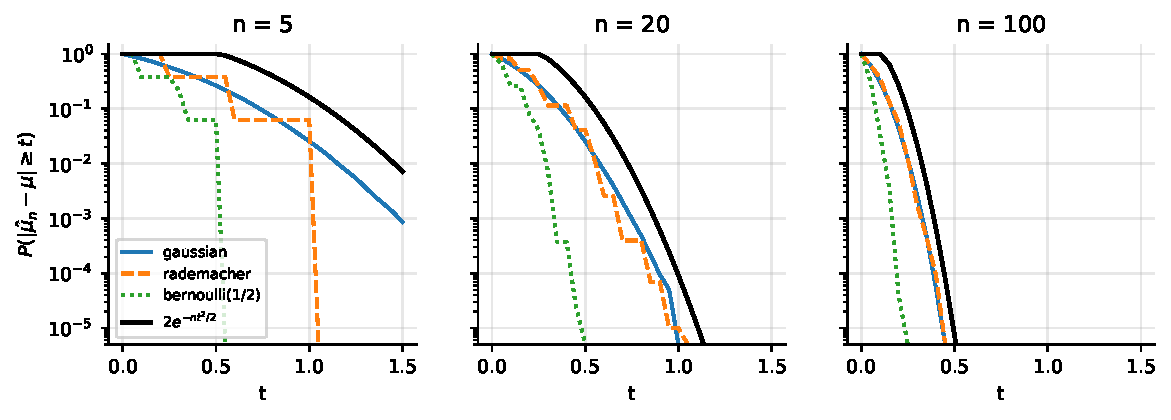
\includegraphics[width=\linewidth]{hoeffding.pdf}
\caption{Empirical tail probabilities (coloured) and the bound $2e^{-nt^2/2}$ (black).}
\label{fig:hoeffding}
\end{figure}

\subsection{(b) Phase-1 regret}

Table~\ref{tab:ucb} and Figure~\ref{fig:ucb} report the phase-1 regret of the UCB rule for $\tau_1\in\{10^3,3\cdot10^3,10^4,3\cdot10^4\}$ and $\Delta\in\{0.1,0.2,0.3,0.5\}$ (means $0.5\pm\Delta/2$). None of the $3{,}200$ runs exceeds bound \eqref{eq:ucb_bound}; the largest regret is $47\%$ of the bound. For $\Delta=0.1$ and $\tau_1\le10^4$ the bound is the trivial $H\Delta$, because $8L_H/\Delta^2$ exceeds $H$. The product $\Delta R(1{:}\tau_1)$ grows linearly in $\log\tau_1$ (right panel), with slope $7.5$--$9.8$ against $8\log(4H^3)/\log H\approx25$ in the bound: the rate $O(\log\tau_1/\Delta)$ is visible, and the constant of the analysis is conservative by a factor of $2.5$ to $3$.

\begin{table}[H]
\centering
\small
\caption{Phase-1 pseudo-regret over 200 runs and the high-probability bound \eqref{eq:ucb_bound} with $\delta=\tau_1^{-2}$.}
\label{tab:ucb}
\begin{tabular}{rrrrrrrr}
\toprule
$\tau_1$ & $\Delta$ & mean & 95\% quantile & max & bound \eqref{eq:ucb_bound} & max $N_j(\tau_1)$ & $1+8L_H/\Delta^2$ \\
\midrule
1,000 & 0.1 & 34.3 & 41.6 & 47.2 & 100.0 & 472 & 17,689 \\
1,000 & 0.3 & 47.3 & 59.1 & 67.2 & 300.0 & 224 & 1,966 \\
1,000 & 0.5 & 43.3 & 53.0 & 60.0 & 354.3 & 120 & 709 \\
10,000 & 0.1 & 171.5 & 211.9 & 251.9 & 1000.0 & 2,519 & 23,215 \\
10,000 & 0.3 & 120.3 & 148.9 & 179.1 & 774.1 & 597 & 2,580 \\
10,000 & 0.5 & 88.5 & 106.0 & 115.5 & 464.8 & 231 & 930 \\
30,000 & 0.1 & 291.0 & 356.5 & 392.3 & 2585.2 & 3,923 & 25,852 \\
30,000 & 0.3 & 157.3 & 189.0 & 234.9 & 862.0 & 783 & 2,873 \\
30,000 & 0.5 & 107.8 & 126.5 & 140.5 & 517.5 & 281 & 1,035 \\
\bottomrule
\end{tabular}
\end{table}

\begin{figure}[H]
\centering
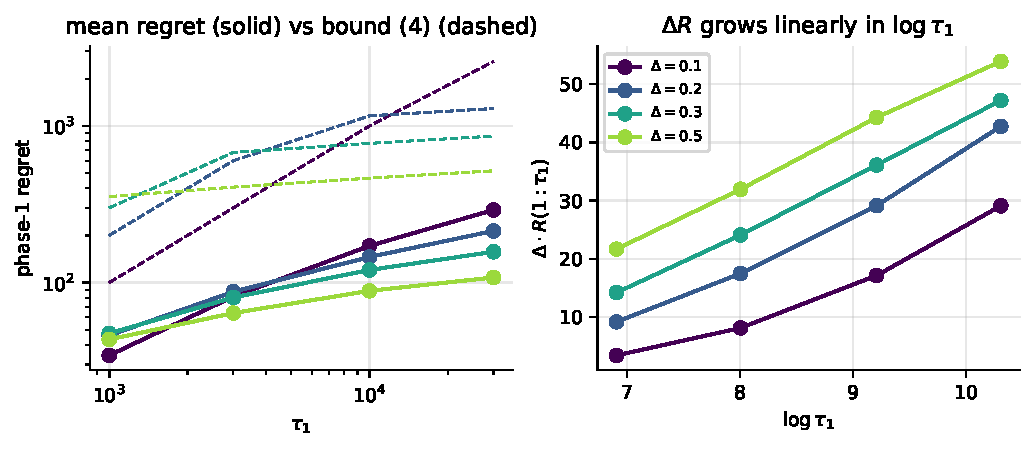
\includegraphics[width=0.9\linewidth]{ucb_phase1.pdf}
\caption{Left: mean phase-1 regret (solid) and bound \eqref{eq:ucb_bound} (dashed). Right: $\Delta\cdot R(1{:}\tau_1)$ against $\log\tau_1$.}
\label{fig:ucb}
\end{figure}

\subsection{(c)(i)--(ii) Window error bounds}

To test \eqref{eq:phase2} and \eqref{eq:phase3} independently of the selection rule, both arms are pulled alternately in scenario S1, so both windows mix samples across both change points. With $\delta=0.05$ and $w\in\{200,1000,3000\}$, no run violates the simultaneous bounds at any round after $\tau_1$ (0 of 200 runs for each $w$); the largest ratio of error to bound is $0.70$, $0.82$ and $0.89$ respectively. The mixing bias computed from the window composition never exceeds the bias terms of \eqref{eq:phase2} and \eqref{eq:phase3} (largest excess $5\times10^{-8}$, single-precision rounding). Figure~\ref{fig:estimation} shows the decomposition: after each change the bias of arm~1 decays linearly in the number of fresh pulls, as in \eqref{eq:alpha}, and reaches zero after $w$ post-change pulls; arm~2 has no bias in phase~2 and a small one after $\tau_2$, where its jump is only $J_{2,2}=0.05$. A longer window lowers the sampling term but stretches the period of bias in proportion to $w$.

\begin{figure}[H]
\centering
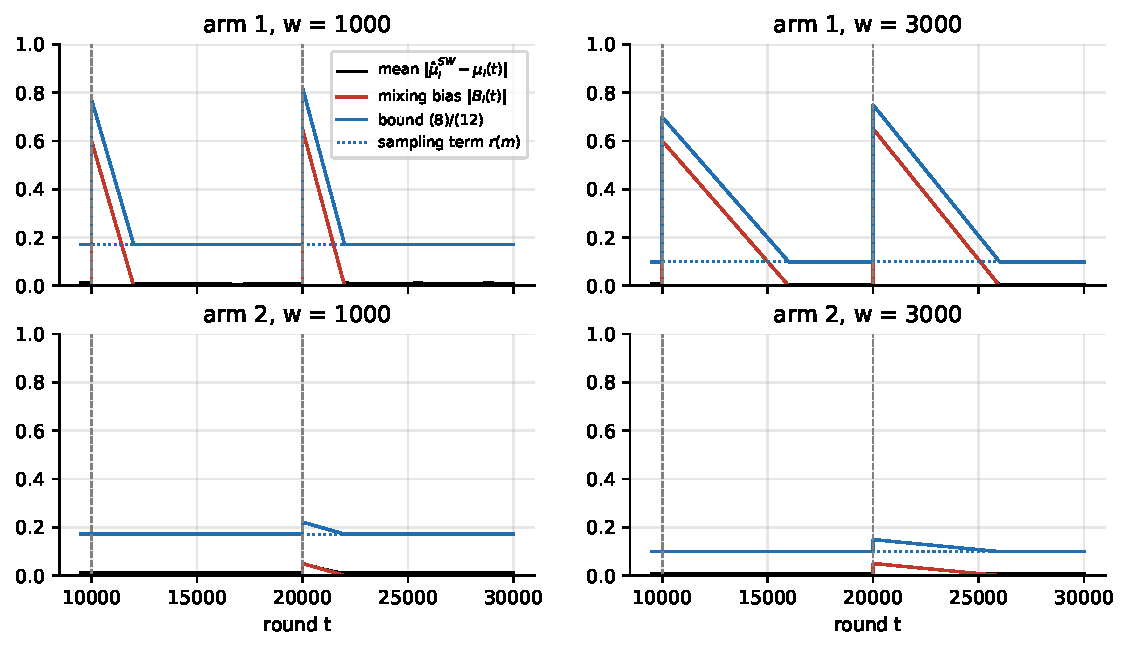
\includegraphics[width=0.95\linewidth]{estimation_bounds.pdf}
\caption{Scenario S1 with alternating pulls: mean absolute error of the window estimate, mixing bias, and the bounds \eqref{eq:phase2}/\eqref{eq:phase3} averaged over 200 runs.}
\label{fig:estimation}
\end{figure}

\subsection{(c)(iii) One window for both change points}

Figure~\ref{fig:window} and Table~\ref{tab:window} report the regret in phases~2 and~3 as a function of $w$. The vertical dotted lines mark the sufficient window $32L_T/g^2$ of \eqref{eq:wprec} ($7{,}824$ for $g=0.3$, $1{,}956$ for $g=0.6$; $70{,}413$ for $g=0.1$ lies outside the plot).

\begin{figure}[H]
\centering
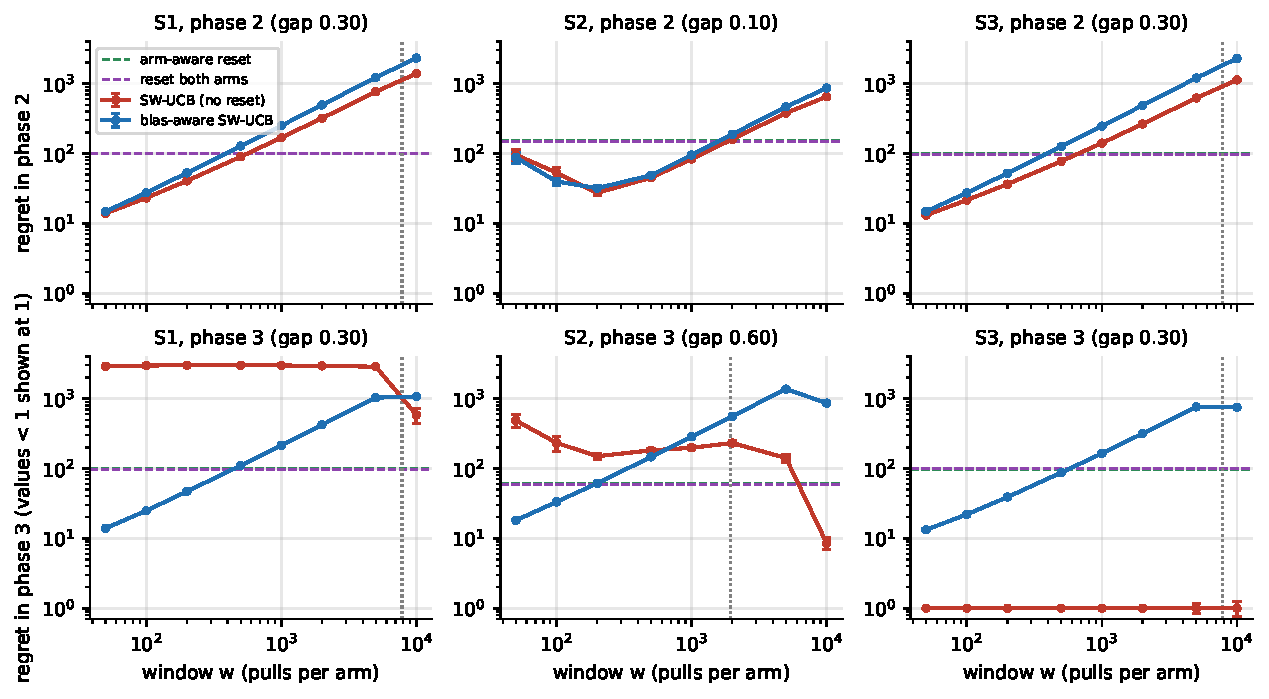
\includegraphics[width=\linewidth]{window_sweep.pdf}
\caption{Regret in phase 2 (top) and phase 3 (bottom) against the window size; dashed lines are the reset variants; 95\% confidence intervals over 200 runs.}
\label{fig:window}
\end{figure}

\begin{table}[H]
\centering
\small
\caption{Best window and regret per phase (mean over 200 runs). For the reset variants the window is unlimited.}
\label{tab:window}
\begin{tabular}{llrrrr}
\toprule
 & & \multicolumn{2}{c}{Phase 2} & \multicolumn{2}{c}{Phase 3} \\
\cmidrule(lr){3-4}\cmidrule(lr){5-6}
Scenario & Policy & best $w$ & regret & best $w$ & regret \\
\midrule
S1 & SW-UCB & 50 & 13.9 & 10,000 & 586.2 \\
 & bias-aware SW-UCB & 50 & 14.8 & 50 & 14.0 \\
 & arm-aware reset & -- & 98.8 & -- & 99.2 \\
\midrule
S2 & SW-UCB & 200 & 27.4 & 10,000 & 8.5 \\
 & bias-aware SW-UCB & 200 & 31.9 & 50 & 18.1 \\
 & arm-aware reset & -- & 154.2 & -- & 60.0 \\
\midrule
S3 & SW-UCB & 50 & 13.1 & any & 0.0 \\
 & bias-aware SW-UCB & 50 & 14.8 & 50 & 13.3 \\
 & arm-aware reset & -- & 100.5 & -- & 96.7 \\
\bottomrule
\end{tabular}
\end{table}

Five observations follow.

\begin{enumerate}
\item \textbf{The window mechanism alone does not guarantee fresh samples.} In S1 and S2 the best arm after $\tau_2$ is arm~1, which was rarely pulled in phase~2. Its window is full of phase-2 observations and does not change while the arm is not selected, so plain SW-UCB keeps the stale ranking: in S1 it pays about $3{,}000$, i.e.\ the full gap in almost every round of phase~3, for every $w\le5{,}000$. This is the requirement stated at the end of part~(c)(iii), and it is not a matter of choosing $w$.
\item \textbf{The confidence radius does not explore when both windows are full.} Once both windows hold $w$ observations, the two radii $r(w)$ are equal and cancel in the comparison of indices, so the rule reduces to comparing window means. Exploration of an unselected arm therefore has to come from elsewhere. The stale-fraction bonus provides it: it is largest for an arm whose window predates its own change, and it vanishes after $w$ fresh pulls. With this bonus the regret in S1 falls from $2{,}907$ to $14$ in phase~3 at $w=50$.
\item \textbf{The sufficient window of \eqref{eq:wprec} is very conservative.} Because the comparison is between window means, the relevant precision is that of the means themselves, of order $\sqrt{\mathrm{Var}/w}$, not the union-bound radius $\sqrt{2L_T/w}$ with $L_T\approx22$. The best windows are $50$--$200$ pulls, one to two orders of magnitude below $32L_T/g^2$, and beyond them regret grows almost linearly in $w$, as the renewal cost \eqref{eq:renewal} predicts.
\item \textbf{Whether one window suffices depends on the gaps.} In S1, where the phase-2 and phase-3 gaps are equal, $w=50$ is best in both phases. In S2 the bias-aware policy is best at $w=200$ in phase~2 (gap $0.1$) and at $w=50$ in phase~3 (gap $0.6$); a common window loses either about $55$ in phase~2 ($w=50$: $87.6$ against $31.9$) or $43$ in phase~3 ($w=200$: $61.2$ against $18.1$). The small gap needs averaging, the large one fast renewal, which is the conflict described in part~(c)(iii).
\item \textbf{A two-arm shift need not be harder.} In S3 both arms move by the same amount and the ranking is unchanged. The stale biases of the two windows have the same sign, and plain SW-UCB has zero regret in phase~3 for every window. The bias-aware policy explores arm~1 because its window is stale, and pays $13$--$761$ for information that is not needed. This is the cancellation described in part~(c)(iii): the jump directions matter, not only the number of arms that change.
\end{enumerate}

The two reset variants have nearly the same regret in all scenarios (within $6$ in every phase). Keeping arm~2's history at $\tau_1$ is worth little here because arm~2 was the worse arm in phase~1 and has few samples to keep. Resets also restart the conservative UCB radius, so their regret ($59$--$154$ per phase) exceeds that of the bias-aware window with a small $w$.

\subsection{(d) Laplace noise}

\paragraph{Coverage of the confidence radius.} Figure~\ref{fig:coverage} compares three radii for means of $n$ Bernoulli$(1/2)$ rewards with added $\mathrm{Laplace}(0,b)$ noise ($4\times10^5$ samples per point): the noise-free radius of part~(a), a radius that only inflates the variance proxy to $1+2b^2$, and the full radius \eqref{eq:rb}. The noise-free radius fails as soon as the noise is non-negligible: at $b=1$ its miscoverage is $1.4$ times $\delta=0.05$ and $10$--$23$ times $\delta=10^{-3}$; at $b=2$ it reaches $174$ times $\delta=10^{-3}$. The variance-only radius is adequate at $\delta=0.05$ but fails in the tail, at $\delta=10^{-3}$ for single observations ($1.3\delta$ for $b=1$, $3.1\delta$ for $b=2$) and for $n=2$ at $b=2$ ($1.4\delta$), because the Laplace distribution is not sub-Gaussian. The full radius \eqref{eq:rb} is valid in all cases, with miscoverage at most $0.04\delta$. This confirms the remark after \eqref{eq:rb}: the linear term $b\log(2/\delta)/n$ is needed.

\begin{figure}[H]
\centering
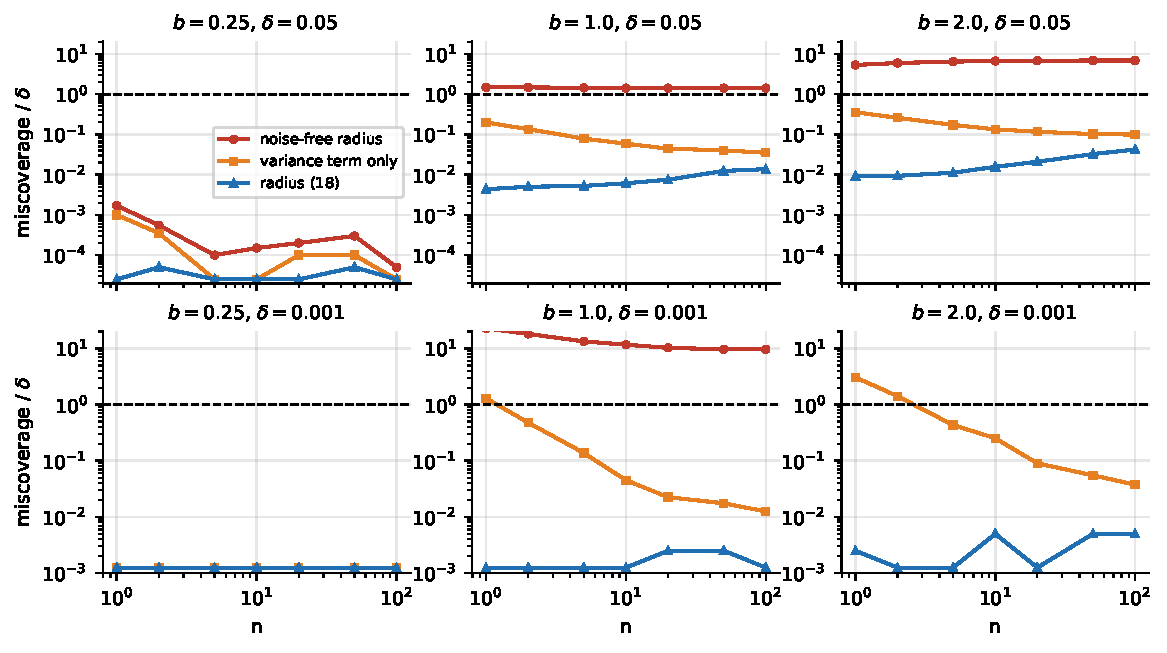
\includegraphics[width=\linewidth]{noise_coverage.pdf}
\caption{Miscoverage divided by $\delta$ (values below the Monte Carlo resolution are shown at the floor); the dashed line is the nominal level.}
\label{fig:coverage}
\end{figure}

\paragraph{Noise shifts the best window upward.} Figure~\ref{fig:noisewindow} repeats the window sweep of scenario S1 for the bias-aware policy with a constant scale $b\in\{0,0.25,0.5,1\}$ and the noisy radius \eqref{eq:noisy_sw}. The window that minimizes the regret after $\tau_1$ grows with the noise: $w=50$ for $b\le0.25$, $100$ for $b=0.5$ and $200$ for $b=1$, where the total regret after $\tau_1$ is $29$, $36$, $70$ and $174$ respectively. Small windows suffer most from the noise ($w=50$: $15\to225$ in phase~2 as $b$ goes from $0$ to $1$), while for $w\ge1{,}000$ the renewal cost dominates and the curves coincide. This is the direction predicted by \eqref{eq:wnoise}: noisier observations require more averaging, at the price of slower renewal.

\begin{figure}[H]
\centering
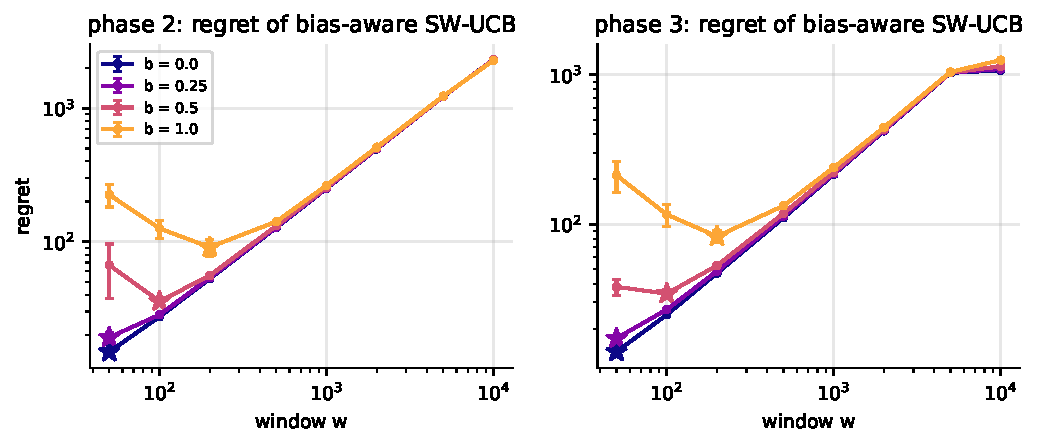
\includegraphics[width=0.9\linewidth]{noise_window.pdf}
\caption{Scenario S1, bias-aware SW-UCB with constant Laplace scale $b$; stars mark the best window.}
\label{fig:noisewindow}
\end{figure}

\paragraph{Allocating a fixed budget.} With $c=1$ and a total budget $E=2T$, uniform spending gives $b_t=0.5$. Following \eqref{eq:blocks}, the horizon is split into three stable blocks and two recovery blocks of $h=2{,}000$ rounds after $\tau_1$ and $\tau_2$; a share $\rho$ of $E$ is spent in the recovery blocks and the rest is spread over the stable blocks in proportion to their lengths ($\rho=2h/T\approx0.13$ is uniform spending). The policy is the bias-aware window with the time-varying radius \eqref{eq:noisy_sw_tv}. Figure~\ref{fig:budget} shows the regret after $\tau_1$ relative to uniform spending. Moderate concentration helps every window: at $\rho=0.25$ (recovery scale $0.27$, stable scale $0.58$) the regret drops by $2.0\%$, $2.5\%$ and $1.6\%$ for $w=300$, $1{,}000$ and $3{,}000$. Stronger concentration helps only the longest window ($-7.1\%$ at $\rho=0.7$ for $w=3{,}000$) and hurts the shorter ones ($+9.6\%$ for $w=300$), whose windows consist mostly of stable-block observations with scale up to $1.44$. This matches the last paragraph of part~(d): budget concentrated around the changes must be balanced against the accuracy of the stable blocks, and the balance depends on $w$. The effects are small in this scenario because the gaps are large compared with the noise; they would grow with smaller budgets or gaps.

\begin{figure}[H]
\centering
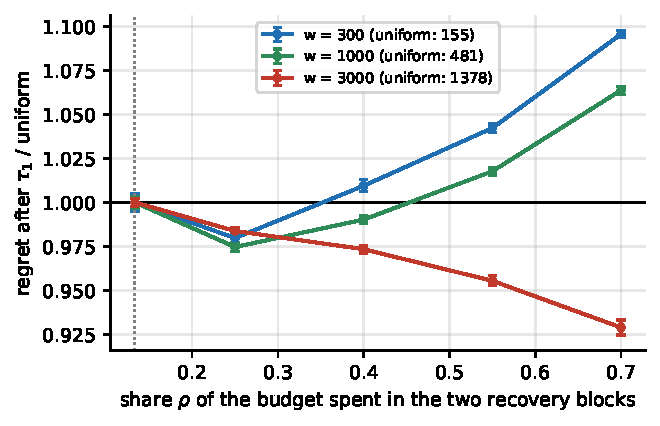
\includegraphics[width=0.6\linewidth]{budget_allocation.pdf}
\caption{Regret after $\tau_1$ relative to uniform spending, as a function of the share of the budget spent in the recovery blocks (dotted line: uniform). 95\% confidence intervals over 200 runs.}
\label{fig:budget}
\end{figure}

\subsection{Summary}

The simulations confirm every bound of the written solution: the Hoeffding bound, the phase-1 regret bound (never exceeded in $3{,}200$ runs, conservative by a factor of $2.5$ to $3$ in its constant), the window error bounds across both change points, and the Laplace confidence radius, whose linear term is needed in the tail. They also sharpen the discussion of part~(c)(iii). A sliding window over pulls must be combined with a mechanism that refreshes stale arms; a bonus equal to the stale fraction of the window, applied only to arms whose mean has changed, does this and uses the asymmetry between the two change points. With that mechanism, a single window suffices when the post-change gaps are comparable but not when they differ, and a common shift of both arms costs nothing to a policy that does not explore. Laplace noise moves the best window upward, and concentrating a fixed budget around the change points helps only up to a point that depends on the window.
